\documentclass[12pt,addpoints,answers]{exam}
\usepackage{amsmath, amssymb, amsthm, enumerate, graphicx}
\usepackage[usenames,dvipsnames]{color}
\usepackage{bm}
\usepackage[colorlinks=true,urlcolor=blue]{hyperref}
\usepackage{geometry}
\geometry{margin=1in}
\usepackage{float}
\usepackage{graphics}
\setlength{\marginparwidth}{2.15cm}
\usepackage{booktabs}
\usepackage{enumitem}
\usepackage{epsfig}
\usepackage{setspace}
\usepackage{parskip}
\usepackage[normalem]{ulem}
\usepackage{tikz}
\usetikzlibrary{positioning, arrows, automata}
\usepackage{pgfplots}
\pgfplotsset{compat=newest}
\usepackage[font=scriptsize]{subcaption}
\usepackage{float}
\usepackage[]{algorithm2e}
\usepackage{environ}
\usepackage{bbm}
\usepackage{graphicx}
\usepackage{titling}
\usepackage{url}
\usepackage{xcolor}
\usepackage{lipsum}
\usepackage{lastpage}
\usepackage[colorlinks=true,urlcolor=blue]{hyperref}
\usepackage{multicol}
\usepackage{tabularx}
\usepackage{comment}
\usepackage[utf8]{inputenc}
\usepackage{amssymb}
\usepackage{setspace}
\usepackage{marvosym}
\usepackage{wrapfig}
\usepackage{datetime}
\usepackage[many]{tcolorbox}
\usepackage{array}
\usepackage{multirow}
\usepackage{wasysym}
\usepackage{cancel}
\usepackage{cprotect}
\usepackage{listings}
\usepackage{color}

%%%%%%%%%%%%%%%%%%%%%%%%%%%%%%%%%%%%%%%%%%%
% Formatting for \CorrectChoice of "exam" %
%%%%%%%%%%%%%%%%%%%%%%%%%%%%%%%%%%%%%%%%%%%

\CorrectChoiceEmphasis{}
\checkedchar{\blackcircle}

\newcommand{\R}{\mathbb{R}}
\newcommand{\blackcircle}{\tikz\draw[black,fill=black] (0,0) circle (1ex);}
\renewcommand{\circle}{\tikz\draw[black] (0,0) circle (1ex);}

\newtcolorbox[]{studentsolution}[1][]{%
    breakable,
    enhanced,
    colback=white,
    title=Solution,
    #1
}

% SOLUTION environment
\NewEnviron{soln}{
\leavevmode\color{red}\ignorespaces \textbf{Solution} \BODY }{}

% QUESTION AUTHORS environment
\NewEnviron{qauthor}{
\leavevmode\color{blue}\ignorespaces \textbf{Author} \BODY}{}

% SOLUTION environment
\NewEnviron{qlearningobjective}{
\leavevmode\color{blue}\ignorespaces \textbf{Learning Objective } \BODY }{}

% TO ONLY SHOW HOMEWORK QUESTIONS, include following (else comment out):
%   \RenewEnviron{soln}{}
 \RenewEnviron{qauthor}{}
 \RenewEnviron{qlearningobjective}{}


%\newcommand{\norm}[1]{\lVert #1 \rVert}
%\newcommand{\st}{\mathrm{s.t.}}

\makeatletter
\newcommand{\removelatexerror}{\let\@latex@error\@gobble}
\makeatother

\newcommand{\argmax}{\mathop{\mathrm{argmax}}}
\newcommand{\argmin}{\mathop{\mathrm{argmin}}}

%%%%%%%%%%%%%%%%%%%%%%%%%%%%%%%%%%%%%%%%%%%
% Custom Math                             %
%%%%%%%%%%%%%%%%%%%%%%%%%%%%%%%%%%%%%%%%%%%

%%%%%%%%%%%%%%%%%%%%%%%%%%%%%%%%%%%%%%%%%%
% Custom commands                        %
%%%%%%%%%%%%%%%%%%%%%%%%%%%%%%%%%%%%%%%%%%

\newcommand{\vc}[1]{\boldsymbol{#1}}
\newcommand{\adj}[1]{\frac{d J}{d #1}}
\newcommand{\chain}[2]{\adj{#2} = \adj{#1}\frac{d #1}{d #2}}

% mathcal
\newcommand{\Ac}{\mathcal{A}}
\newcommand{\Bc}{\mathcal{B}}
\newcommand{\Cc}{\mathcal{C}}
\newcommand{\Dc}{\mathcal{D}}
\newcommand{\Ec}{\mathcal{E}}
\newcommand{\Fc}{\mathcal{F}}
\newcommand{\Gc}{\mathcal{G}}
\newcommand{\Hc}{\mathcal{H}}
\newcommand{\Ic}{\mathcal{I}}
\newcommand{\Jc}{\mathcal{J}}
\newcommand{\Kc}{\mathcal{K}}
\newcommand{\Lc}{\mathcal{L}}
\newcommand{\Mc}{\mathcal{M}}
\newcommand{\Nc}{\mathcal{N}}
\newcommand{\Oc}{\mathcal{O}}
\newcommand{\Pc}{\mathcal{P}}
\newcommand{\Qc}{\mathcal{Q}}
\newcommand{\Rc}{\mathcal{R}}
\newcommand{\Sc}{\mathcal{S}}
\newcommand{\Tc}{\mathcal{T}}
\newcommand{\Uc}{\mathcal{U}}
\newcommand{\Vc}{\mathcal{V}}
\newcommand{\Wc}{\mathcal{W}}
\newcommand{\Xc}{\mathcal{X}}
\newcommand{\Yc}{\mathcal{Y}}
\newcommand{\Zc}{\mathcal{Z}}

% mathbb
\newcommand{\Ab}{\mathbb{A}}
\newcommand{\Bb}{\mathbb{B}}
\newcommand{\Cb}{\mathbb{C}}
\newcommand{\Db}{\mathbb{D}}
\newcommand{\Eb}{\mathbb{E}}
\newcommand{\Fb}{\mathbb{F}}
\newcommand{\Gb}{\mathbb{G}}
\newcommand{\Hb}{\mathbb{H}}
\newcommand{\Ib}{\mathbb{I}}
\newcommand{\Jb}{\mathbb{J}}
\newcommand{\Kb}{\mathbb{K}}
\newcommand{\Lb}{\mathbb{L}}
\newcommand{\Mb}{\mathbb{M}}
\newcommand{\Nb}{\mathbb{N}}
\newcommand{\Ob}{\mathbb{O}}
\newcommand{\Pb}{\mathbb{P}}
\newcommand{\Qb}{\mathbb{Q}}
\newcommand{\Rb}{\mathbb{R}}
\newcommand{\Sb}{\mathbb{S}}
\newcommand{\Tb}{\mathbb{T}}
\newcommand{\Ub}{\mathbb{U}}
\newcommand{\Vb}{\mathbb{V}}
\newcommand{\Wb}{\mathbb{W}}
\newcommand{\Xb}{\mathbb{X}}
\newcommand{\Yb}{\mathbb{Y}}
\newcommand{\Zb}{\mathbb{Z}}

% mathbf lowercase
\newcommand{\av}{\mathbf{a}}
\newcommand{\bv}{\mathbf{b}}
\newcommand{\cv}{\mathbf{c}}
\newcommand{\dv}{\mathbf{d}}
\newcommand{\ev}{\mathbf{e}}
\newcommand{\fv}{\mathbf{f}}
\newcommand{\gv}{\mathbf{g}}
\newcommand{\hv}{\mathbf{h}}
\newcommand{\iv}{\mathbf{i}}
\newcommand{\jv}{\mathbf{j}}
\newcommand{\kv}{\mathbf{k}}
\newcommand{\lv}{\mathbf{l}}
\newcommand{\mv}{\mathbf{m}}
\newcommand{\nv}{\mathbf{n}}
\newcommand{\ov}{\mathbf{o}}
\newcommand{\pv}{\mathbf{p}}
\newcommand{\qv}{\mathbf{q}}
\newcommand{\rv}{\mathbf{r}}
\newcommand{\sv}{\mathbf{s}}
\newcommand{\tv}{\mathbf{t}}
\newcommand{\uv}{\mathbf{u}}
\newcommand{\vv}{\mathbf{v}}
\newcommand{\wv}{\mathbf{w}}
\newcommand{\xv}{\mathbf{x}}
\newcommand{\yv}{\mathbf{y}}
\newcommand{\zv}{\mathbf{z}}

% mathbf uppercase
\newcommand{\Av}{\mathbf{A}}
\newcommand{\Bv}{\mathbf{B}}
\newcommand{\Cv}{\mathbf{C}}
\newcommand{\Dv}{\mathbf{D}}
\newcommand{\Ev}{\mathbf{E}}
\newcommand{\Fv}{\mathbf{F}}
\newcommand{\Gv}{\mathbf{G}}
\newcommand{\Hv}{\mathbf{H}}
\newcommand{\Iv}{\mathbf{I}}
\newcommand{\Jv}{\mathbf{J}}
\newcommand{\Kv}{\mathbf{K}}
\newcommand{\Lv}{\mathbf{L}}
\newcommand{\Mv}{\mathbf{M}}
\newcommand{\Nv}{\mathbf{N}}
\newcommand{\Ov}{\mathbf{O}}
\newcommand{\Pv}{\mathbf{P}}
\newcommand{\Qv}{\mathbf{Q}}
\newcommand{\Rv}{\mathbf{R}}
\newcommand{\Sv}{\mathbf{S}}
\newcommand{\Tv}{\mathbf{T}}
\newcommand{\Uv}{\mathbf{U}}
\newcommand{\Vv}{\mathbf{V}}
\newcommand{\Wv}{\mathbf{W}}
\newcommand{\Xv}{\mathbf{X}}
\newcommand{\Yv}{\mathbf{Y}}
\newcommand{\Zv}{\mathbf{Z}}

% bold greek lowercase
\newcommand{\alphav     }{\boldsymbol \alpha     }
\newcommand{\betav      }{\boldsymbol \beta      }
\newcommand{\gammav     }{\boldsymbol \gamma     }
\newcommand{\deltav     }{\boldsymbol \delta     }
\newcommand{\epsilonv   }{\boldsymbol \epsilon   }
\newcommand{\varepsilonv}{\boldsymbol \varepsilon}
\newcommand{\zetav      }{\boldsymbol \zeta      }
\newcommand{\etav       }{\boldsymbol \eta       }
\newcommand{\thetav     }{\boldsymbol \theta     }
\newcommand{\varthetav  }{\boldsymbol \vartheta  }
\newcommand{\iotav      }{\boldsymbol \iota      }
\newcommand{\kappav     }{\boldsymbol \kappa     }
\newcommand{\varkappav  }{\boldsymbol \varkappa  }
\newcommand{\lambdav    }{\boldsymbol \lambda    }
\newcommand{\muv        }{\boldsymbol \mu        }
\newcommand{\nuv        }{\boldsymbol \nu        }
\newcommand{\xiv        }{\boldsymbol \xi        }
\newcommand{\omicronv   }{\boldsymbol \omicron   }
\newcommand{\piv        }{\boldsymbol \pi        }
\newcommand{\varpiv     }{\boldsymbol \varpi     }
\newcommand{\rhov       }{\boldsymbol \rho       }
\newcommand{\varrhov    }{\boldsymbol \varrho    }
\newcommand{\sigmav     }{\boldsymbol \sigma     }
\newcommand{\varsigmav  }{\boldsymbol \varsigma  }
\newcommand{\tauv       }{\boldsymbol \tau       }
\newcommand{\upsilonv   }{\boldsymbol \upsilon   }
\newcommand{\phiv       }{\boldsymbol \phi       }
\newcommand{\varphiv    }{\boldsymbol \varphi    }
\newcommand{\chiv       }{\boldsymbol \chi       }
\newcommand{\psiv       }{\boldsymbol \psi       }
\newcommand{\omegav     }{\boldsymbol \omega     }

% bold greek uppercase
\newcommand{\Gammav     }{\boldsymbol \Gamma     }
\newcommand{\Deltav     }{\boldsymbol \Delta     }
\newcommand{\Thetav     }{\boldsymbol \Theta     }
\newcommand{\Lambdav    }{\boldsymbol \Lambda    }
\newcommand{\Xiv        }{\boldsymbol \Xi        }
\newcommand{\Piv        }{\boldsymbol \Pi        }
\newcommand{\Sigmav     }{\boldsymbol \Sigma     }
\newcommand{\Upsilonv   }{\boldsymbol \Upsilon   }
\newcommand{\Phiv       }{\boldsymbol \Phi       }
\newcommand{\Psiv       }{\boldsymbol \Psi       }
\newcommand{\Omegav     }{\boldsymbol \Omega     }

%%%%%%%%%%%%%%%%%%%%%%%%%%%%%%%%%%%%%%%%%%%
% Custom box for highlights               %
%%%%%%%%%%%%%%%%%%%%%%%%%%%%%%%%%%%%%%%%%%%

% Define box and box title style
\tikzstyle{mybox} = [fill=blue!10, very thick,
    rectangle, rounded corners, inner sep=1em, inner ysep=1em]

% \newcommand{\notebox}[1]{
% \begin{tikzpicture}
% \node [mybox] (box){%
%     \begin{minipage}{\textwidth}
%     #1
%     \end{minipage}
% };
% \end{tikzpicture}%
% }

\NewEnviron{notebox}{

\begin{tikzpicture}
\node [mybox] (box){
    \begin{minipage}{\textwidth}
        \BODY
    \end{minipage}
};
\end{tikzpicture}
}


\begin{document}
\section*{}
\begin{center}
  \centerline{\textsc{\LARGE  Homework 6}}
  \vspace{0.5em}
  \centerline{\textsc{\LARGE Learning Theory and Generative Models}\footnote{Compiled on \today{} at \currenttime{}}}
  \vspace{1em}
  \textsc{\large CMU 10-301/10-601: Machine Learning (Spring 2020)} \\
  \vspace{0.5em}
  \url{https://piazza.com/cmu/spring2020/1030110601/} \\
  \vspace{0.5em}
  \centerline{OUT: Friday, Mar 20th, 2020}
  %\today{} at \currenttime{}}}
  \vspace{0.5em}
  \centerline{DUE: Friday, Mar 27th, 2020, 11:59pm}
    \centerline{TAs: Sankalp Patro, Vinay Sameer Kadi, Hanyue Chai, Sana Lakdawala, Vishal Baskar}
\end{center}


\section*{START HERE: Instructions}

\begin{notebox}
Homework 6 covers topics on learning theory, MLE/MAP, Naive Bayes, and revisits neural networks, logistic regression and regularization. The homework includes multiple choice, True/False, and short answer questions. 
\end{notebox}

\begin{itemize}
\item \textbf{Collaboration policy:} Collaboration on solving the homework is allowed, after you have thought about the problems on your own. It is also OK to get clarification (but not solutions) from books or online resources, again after you have thought about the problems on your own. There are two requirements: first, cite your collaborators fully and completely (e.g., ``Jane explained to me what is asked in Question 2.1''). Second, write your solution {\em independently}: close the book and all of your notes, and send collaborators out of the room, so that the solution comes from you only.  See the Academic Integrity Section on the course site for more information: \url{http://www.cs.cmu.edu/~mgormley/courses/10601/about.html#7-academic-integrity-policies}

\item\textbf{Late Submission Policy:} See the late submission policy here: \url{http://www.cs.cmu.edu/~mgormley/courses/10601/about.html#6-general-policies}

\item\textbf{Submitting your work:} 

\begin{itemize}

\item \textbf{Gradescope:} For written problems such as short answer, multiple choice, derivations, proofs, or plots, we will be using Gradescope (\url{https://gradescope.com/}). Please use the provided template. Submissions can be handwritten onto the template, but should be labeled and clearly legible. If your writing is not legible, you will not be awarded marks. Alternatively, submissions can be written in LaTeX. Regrade requests can be made, however this gives the TA the opportunity to regrade your entire paper, meaning if additional mistakes are found then points will be deducted.
Each derivation/proof should be completed on a separate page. For short answer questions, you \textbf{should not} include your work in your solution.  If you include your work in your solutions, your assignment may not be graded correctly by our AI assisted grader. In addition, please tag the problems to the corresponding pages when submitting your work.

\end{itemize}

% \item \textbf{Materials:} Download from autolab the tar file (``Download handout"). The tar file will contain all the data that you will need in order to complete this assignment.

\end{itemize}

For multiple choice or select all that apply questions, shade in the box or circle in the template document corresponding to the correct answer(s) for each of the questions. For \LaTeX users, use $\blacksquare$ and \blackcircle  for shaded boxes and circles, and don't change anything else.

\clearpage

\section*{Instructions for Specific Problem Types}

For ``Select One" questions, please fill in the appropriate bubble completely:

\begin{quote}
\textbf{Select One:} Who taught this course?
\begin{checkboxes}
     \CorrectChoice Matt Gormley
     \choice Marie Curie
     \choice Noam Chomsky
\end{checkboxes}
\end{quote}

If you need to change your answer, you may cross out the previous answer and bubble in the new answer:

\begin{quote}
\textbf{Select One:} Who taught this course?
\begin{list}{}
     \item\CIRCLE{} Matt Gormley
     \item\Circle{} Marie Curie\\
     \xcancel{\CIRCLE}{} Noam Chomsky
\end{list}
\end{quote}


For ``Select all that apply" questions, please fill in all appropriate squares completely:

\begin{quote}
\textbf{Select all that apply:} Which are scientists?
{
    \checkboxchar{$\Box$} \checkedchar{$\blacksquare$}
    \begin{checkboxes}
     \choice Stephen Hawking 
     \CorrectChoice Albert Einstein
     \choice Isaac Newton
     \choice None of the above
    \end{checkboxes}
    }
\end{quote}

Again, if you need to change your answer, you may cross out the previous answer(s) and bubble in the new answer(s):

\begin{quote}
\textbf{Select all that apply:} Which are scientists?
    \begin{list}{}
    \item $\blacksquare$ Stephen Hawking 
    \item $\blacksquare$ Albert Einstein
    \item $\blacksquare$ Isaac Newton\\
    \xcancel{$\blacksquare$} I don't know
\end{list}
\end{quote}

For questions where you must fill in a blank, please make sure your final answer is fully included in the given space. You may cross out answers or parts of answers, but the final answer must still be within the given space.

\begin{quote}
\textbf{Fill in the blank:} What is the course number?

\begin{tcolorbox}[fit,height=1cm, width=4cm, blank, borderline={1pt}{-2pt},nobeforeafter]
    \begin{center}\huge10-601\end{center}
    \end{tcolorbox}\hspace{2cm}
    \begin{tcolorbox}[fit,height=1cm, width=4cm, blank, borderline={1pt}{-2pt},nobeforeafter]
    \begin{center}\huge10-\xcancel{7}601\end{center}
    \end{tcolorbox}
\end{quote}

\clearpage

\section{Neural Networks, Logistic Regression, Regularization Revisited [28 pts]}

    \textbf{} Imagine you work for a pharmaceutical company that is trying to predict whether certain patients will respond well to a new drug. Specifically, these patients have high blood pressure in their lungs, a condition known as pulmonary hypertension. Doctors recommend that the best predictors of a treatment effect is the patient's heart function (measured by cardiac output) and the blood pressure in their lungs (pulmonary blood pressure). You plot the data and visualize the following:
    
        \begin{figure}[H]
        \centering
        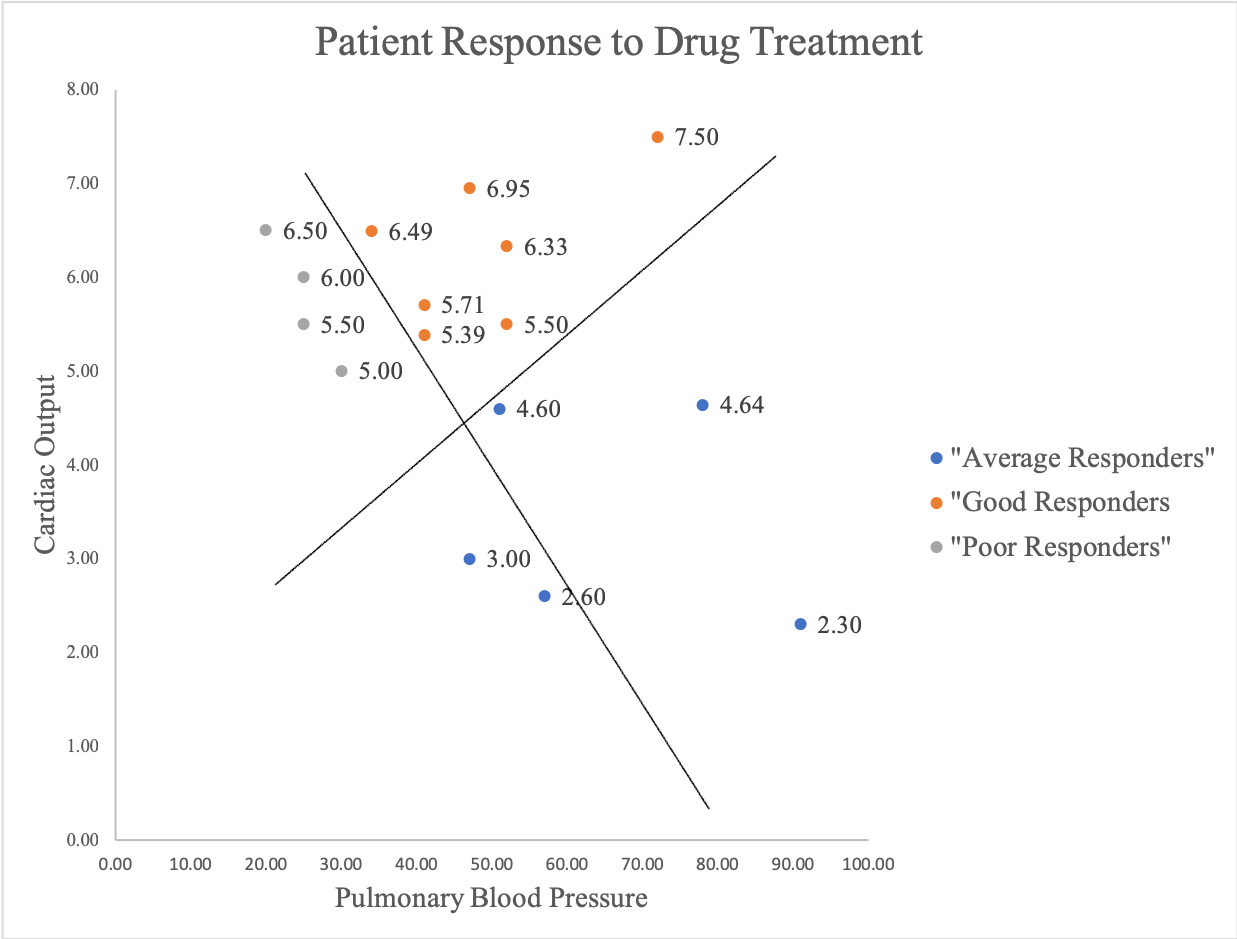
\includegraphics[width=1\textwidth]{patients.png}
        \end{figure}
\begin{enumerate}        
    \item {\textbf{[3 pt]}} Draw on the graph above the decision boundaries of a trained neural network that minimizes the training error when classifying Good Responders vs all others (Poor or Average). Assume the neural network has two hidden units and one hidden layer. What is the smallest training error you can achieve?
    
        \textbf{Fill in the blank (write answer as a fraction):}
    
    \begin{tcolorbox}[fit,height=1cm, width=4cm, blank, borderline={1pt}{-2pt},nobeforeafter]
    \end{tcolorbox}
    
    
    \item {\textbf{[2 pt]}} Using your decision boundaries above, assuming a logistic activation function, which point has the highest probability of being a Good Responder? Provide the point number as shown on the graph (poitnts are labeled by their y value).
    
            \textbf{Fill in the blank:}
    
    \begin{tcolorbox}[fit,height=1cm, width=4cm, blank, borderline={1pt}{-2pt},nobeforeafter]
    \end{tcolorbox}
    
    
    \item {\textbf{[2 pt]}} True or False: Increasing the number of hidden units of a neural network will always guarantee a lower training error. 
    
        \begin{checkboxes}
        \choice True
        \choice False
        \end{checkboxes}
    
    
    \item {\textbf{[2 pt]}} When performing linear regression, which of the following options will decrease mean-squared training error:
    
    \textbf{Select all that apply:}
    {\checkboxchar{$\Box$} \checkedchar{$\blacksquare$}
        \begin{checkboxes}
        \choice Increasing the order of the polynomial
        \choice Increasing the regularization weight
        \choice For the same weight on the regularizer, using an L1 regularizer instead of an L2
        \choice For the same weight on the regularizer, using an L1 regularizer instead of an L0
        \choice None of the above
        \end{checkboxes}
    }


    \item {\textbf{[2 pt]}} Convolutional neural networks often consist of convolutional layers, max-pooling layers, and fully-connected layers. Select all the layer types below that have parameters (i.e. weights) which can be learned by gradient descent / backpropagation.
    
    \textbf{Select all that apply:}
    {\checkboxchar{$\Box$} \checkedchar{$\blacksquare$}
        \begin{checkboxes}
            \choice convolutional layer
            \choice max-pooling layer
            \choice fully-connected layer
        \end{checkboxes}
    }
    
    \clearpage
    
    \item {\textbf{[3 pt]}} Consider the black-and-white 5 pixel by 5 pixel image shown below. Black pixels are represented by the value 0 and white pixels by 1.
    
    \begin{center}
    \begin{tabular}{|c|c|c|c|c|}
    \hline
    1 & 1 & 0 & 0 & 0    \\ \hline
    1 & 1 & 1 & 0 & 0    \\ \hline
    0 & 1 & 1 & 1 & 0     \\ \hline
    0 & 0 & 1 & 1 & 1     \\ \hline
    0 & 0 & 0 & 1 & 1     \\ \hline
    \end{tabular}
    \end{center}
    
    Next consider the 3 by 3 convolution with weights shown below.

    \begin{center}
    \begin{tabular}{|c|c|c|}
    \hline
    -1 & 0 & 1    \\ \hline
    -1 & 0 & 1    \\ \hline
    -1 & 0 & 1     \\ \hline
    \end{tabular}
    \end{center}

    Suppose we apply the above convolution (as one would in a CNN convolutional layer) to the above image to produce a new output image. Assume that we do not permit any padding to be used and the stride of the convolution is 1. What is the value of the pixel in the upper-left corner of the output image?
    
    
    (Important Note: Convolution is sometimes defined differently in machine learning than in other fields, such as signal processing. So be sure to follow the method of convolution shown in the guest lecture on CNNs.)
    
        \textbf{Fill in the blank:}
    
    \begin{tcolorbox}[fit,height=1cm, width=4cm, blank, borderline={1pt}{-2pt},nobeforeafter]
    
    %solution
    \end{tcolorbox}   
    
    
    \item {\textbf{[3 pt]}} For the same output image produced in the previous question, what is the value of the pixel in the upper-right corner of the output image?
    
        \textbf{Fill in the blank:}
    
    \begin{tcolorbox}[fit,height=1cm, width=4cm, blank, borderline={1pt}{-2pt},nobeforeafter]
    
    %solution
    \end{tcolorbox}   
    
    
    \item {\textbf{[2 pt]}} True or False: Long Short Term Memory (LSTM) networks partially address the vanishing gradient problem by incorporating input, output, and forget gates.
        \begin{checkboxes}
            \choice True
            \choice False
        \end{checkboxes}
    
    
    \item {\textbf{[2 pt]}} True or False: In a recurrent neural network (RNN), the weight vector passed to a hidden unit at the same hidden layer level from a prior unit will have different values.
        \begin{checkboxes}
            \choice True
            \choice False
        \end{checkboxes}
    
    \clearpage
    
    \item {\textbf{[2 pt]}} True or False: Recurrent neural networks (RNNs) can accept sequence data as input, but can only output a single classification decision for that input sequence.
        \begin{checkboxes}
            \choice True
            \choice False
        \end{checkboxes}
    
        
    \item \textbf{[2 pt]} Which of the following are true about regularization?
    \textbf{Select all that apply:}
    {%
    \checkboxchar{$\Box$} \checkedchar{$\blacksquare$}
    \begin{checkboxes}
        \choice One of the goals of regularization is combating overfitting.  
        \choice A model with regularization fits the training data better than a model without regularization 
        \choice The L-0 norm (number of non-zero parameters) is rarely used in practice in part because it is non-differentiable. 
        \choice One way to understand regularization is that it attempts to follow Occam's razor and make the learning algorithm prefer "simpler" solutions.
    \end{checkboxes}
    }
    
    \item \textbf{[3 pt]} When performing linear regression, which of the following options will decrease mean-squared training error:
    
    \textbf{Select all that apply:}
        {%
    \checkboxchar{$\Box$} \checkedchar{$\blacksquare$}
        \begin{checkboxes}
        \choice Adding higher-order functions of the features as separate features
        \choice Increasing the regularization weight
        \choice For the same weight on the regularizer, using an L1 regularizer instead of an L2
        \choice For the same weight on the regularizer, using an L1 regularizer instead of an L0
        \choice None of the above
        \end{checkboxes}
        }

    
\end{enumerate}




\clearpage
\section{Learning Theory [18 pts]}
\begin{enumerate}
    \item \textbf{[3 pt]} Let $\delta=|H|e^{-\epsilon m}$. According to the PAC theorems discussed in class, which of the following is correct? Select one.

    \textbf{Select one:}
    \begin{checkboxes}
        \choice With probability at least $1- \delta$, every hypothesis with training error at most $\epsilon$ has true error 0.
        \choice With probability at least $1-\epsilon$, a random hypothesis with training error 0 has true error at most $\delta$.
        \choice With probability at least $1-\delta$, every hypothesis with training error 0 has true error at most $\epsilon$.
        \choice With probability at least $1-\epsilon$, a random hypothesis with true error 0 has training error at most $\delta$.
    \end{checkboxes}
    
    
    \item \textbf{[3 pt]} Consider a decision tree learner applied to data where each example is described by 10 boolean variables $X_1, X_2, \cdots, X_{10}$. What is the VC dimension of the hypothesis space used by this decision tree learner?
    
    \textbf{Fill in the blank:}
    
    \begin{tcolorbox}[fit,height=1cm, width=4cm, blank, borderline={1pt}{-2pt},nobeforeafter]
    
    %solution
    \end{tcolorbox}   
    
    
    \item \textbf{[4 pt]} Consider instance space X which is the set of real numbers. What is the VC dimension of hypothesis class $H$, where each hypothesis $h$ in $H$ is of the form  ``if a $<$ x $<$ b or c $<$ x $<$ d then y = 1; otherwise y = 0"?  (i.e., H is an infinite hypothesis class where a, b, c, and d are arbitrary real numbers.

    \textbf{Select one:}
    \begin{checkboxes}
        \choice 2
        \choice 3
        \choice 4
        \choice 5
        \choice 6
    \end{checkboxes}
    

    \clearpage
    
    \item \textbf{[3 pt]} Alex is given a classification task to solve. He has no idea where to start, so he decided to try out a decision tree learner with 2 binary features $X_1$ and $X_2$. He recently learned about PAC learning, and would like to know what is the minimum number (N) of data points that would suffice for the PAC criterion with $\epsilon = 0.1$ and $\delta = 0.01$. 
    
    Notice that a valid decision tree may or may not be full, meaning it doesn't have to split on all features.
    
    \textbf{Fill in the blank:}
    
    \begin{tcolorbox}[fit,height=1cm, width=4cm, blank, borderline={1pt}{-2pt},nobeforeafter]
    
    %solution
    \end{tcolorbox} 
    
    
    
    \item \textbf{[2 pt]} Sally thinks Alex shouldn't have used a decision tree with 2 binary features. Instead, she thinks it would be best to use logistic regression with 16 real-valued features in addition to a bias term. Sally overherd Alex talking about this cool concept called PAC learning and she too would like to use it to analyze her method. She first trains her logistic regression model on $N$ examples to obtain a training error $\hat R$. What is the the upper bound on the true error $R$ in terms of $\hat R$, $\delta$, and $N$. You may use big-$\mathcal{O}$ notation.
    
    \textbf{Fill in the blank:}
    
    \begin{tcolorbox}[fit,height=1cm, width=15cm, blank, borderline={1pt}{-2pt},nobeforeafter]
    
    %solution
    \end{tcolorbox} 
    
    
    \item \textbf{[3 pt]} Sally wants to argue her method has lower bound on the true error. Assuming Sally has obtained enough data points to satisfy PAC criterion with $\epsilon = 0.1$ and $\delta = 0.01$. Which of the following is true?
    
    \textbf{Select one:}
    \begin{checkboxes}
        \choice Sally is wrong. Alex's method will always classify unseen data more accurately since it is simpler as it only needs 2 binary features.
        \choice She must first regularize her model by removing 14 features to make any comparison at all.
        \choice It is sufficient to show that the VC Dimension of her classifier is higher than Alex's, therefore having lower bound for the true error.
        \choice It is necessary to show that the training error she achieves is lower than the training error Alex achieves.
    \end{checkboxes}
    
    
    \clearpage
    
    
    
\end{enumerate}

\clearpage

\section{MLE/MAP [34 pts]}
\begin{enumerate}

    \item \textbf{[3 pt]} \textbf{True or False:} Suppose you place a Beta prior over the Bernoulli distribution, and attempt to learn the parameter of the Bernoulli distribution from data. Further suppose an adversary chooses ``bad", but finite hyperparameters for your Beta prior in order to confuse your learning algorithm. As the number of training examples grows to infinity, the MAP estimate of $\theta$ can still converge to the MLE estimate of $\theta$.
    
    \textbf{Select One:}
    
    \begin{checkboxes}
        \choice True
        \choice False
    \end{checkboxes}
    
    
    \item \textbf{[3 pt]} Let $\theta$ be a random variable with the following probability density function (pdf): 
    \begin{align*}
        f(\theta) &= 
        \begin{cases}
        2\theta  & \text{if } 0 \leq \theta \leq 1 \\
        0  & \text{otherwise}
        \end{cases}
    \end{align*}
    
    Suppose another random variable Y, which is conditioning on $\theta$, follows an exponential distribution with  $\lambda=3\theta$. Recall that the exponential distribution with parameter $\lambda$ has the following pdf:
    
    %$f(y)=\lambda e^{-\lambda y}$ if $y\geq 0$, otherwise $f(y)=0$
    
    \begin{align*}
        f_{exp}(y) &= 
        \begin{cases}
        \lambda e^{-\lambda y}  & \text{if } y\geq 0 \\
        0  & \text{otherwise}
        \end{cases}
    \end{align*}
    
    What is the MAP estimate of $\theta$ given $Y=\frac{2}{3}$ is observed?

    \textbf{Select one:}
    \begin{checkboxes}
        \choice 0
        \choice 1/3
        \choice 1
        \choice 2
    \end{checkboxes}
    
    
    \clearpage
    
    \item \textbf{[3 pt]} In HW3, you have derived the closed form solution for linear regression. Now, we are coming back to linear regression, viewing it as a statistical model, and deriving the MLE and MAP estimate of the parameters in the following questions. 
    
    Assume we have data $D = \{\mathbf{x}^{(i)}, y^{(i)}\}_{i=1}^{N}$, where $\mathbf{x}^{(i)} = (x_1^{(i)}, \cdots, x_M^{(i)})$ . So our data has $N$  instances and each instance has $M$  attributes/features. Each $y^{(i)}$ is generated given $\mathbf{x}^{(i)}$ with additive noise $\epsilon^{(i)} \sim N(0, \sigma^2)$, that is $y^{(i)} = \mathbf{w}^T \mathbf{x}^{(i)} + \epsilon^{(i)}$ where $\mathbf{w}$  is the parameter vector of linear regression. Given this assumption, what is the distribution of y? 

    \textbf{Select one:}
    \begin{checkboxes}
        \choice $y^{(i)} \sim N(\mathbf{w}^T \mathbf{x}^{(i)}, \sigma^2)$
        \choice $y^{(i)} \sim N(0, \sigma^2)$
        \choice $y^{(i)} \sim \textit{Uniform}(\mathbf{w}^T \mathbf{x}^{(i)} - \sigma,  \mathbf{w}^T \mathbf{x}^{(i)} + \sigma)$
        \choice None of the above
    \end{checkboxes}
    
    
    \item \textbf{[4 pt]} The next step is to learn the MLE of the parameters of the linear regression model. Which expression below is the correct conditional log likelihood $\ell(\mathbf{w})$ with the given data?

    \textbf{Select one:}
    \begin{checkboxes}
        \choice $\sum_{i=1}^{N} [-\log (\sqrt{2\pi\sigma^2}) - \frac{1}{2\sigma^2} (y^{(i)} - \mathbf{w}^T\mathbf{x}^{(i)})^2]$
        \choice $\sum_{i=1}^{N} [\log (\sqrt{2\pi\sigma^2}) + \frac{1}{2\sigma^2} (y^{(i)} - \mathbf{w}^T\mathbf{x}^{(i)})^2]$
        \choice $\sum_{i=1}^{N} [-\log(\sqrt{2\pi\sigma^2)} - \frac{1}{2\sigma^2} (y^{(i)} - \mathbf{w}^T\mathbf{x}^{(i)})]$
        \choice $-\log (\sqrt{2\pi\sigma^2}) + \sum_{i=1}^{N} [-\frac{1}{2\sigma^2} (y^{(i)} - \mathbf{w}^T\mathbf{x}^{(i)})^2]$
    \end{checkboxes}
    
    
    \item \textbf{[4 pt]} Then, the MLE of the parameters is just  $\argmax_{\mathbf{w}} \ell(\mathbf{w})$ . Among the following expressions, select ALL that can yield the correct MLE. 

    \textbf{Select all that apply:}
    {\checkboxchar{$\Box$} \checkedchar{$\blacksquare$}
        \begin{checkboxes}
        \choice $\argmax_{\mathbf{w}} \sum_{i=1}^{N} [-\log (\sqrt{2\pi\sigma^2}) - \frac{1}{2\sigma^2} (y^{(i)} - \mathbf{w}^T\mathbf{x}^{(i)})]$
        \choice $\argmax_{\mathbf{w}} \sum_{i=1}^{N} [-\log (\sqrt{2\pi\sigma^2}) - \frac{1}{2\sigma^2} (y^{(i)} - \mathbf{w}^T\mathbf{x}^{(i)})^2]$
        \choice $\argmax_{\mathbf{w}} \sum_{i=1}^{N} [- \frac{1}{2\sigma^2} (y^{(i)} - \mathbf{w}^T\mathbf{x}^{(i)})^2]$
        \choice $\argmax_{\mathbf{w}} \sum_{i=1}^{N} [- \frac{1}{2} (y^{(i)} - \mathbf{w}^T\mathbf{x}^{(i)})]$
        \choice $\argmax_{\mathbf{w}} \sum_{i=1}^{N} [- \frac{1}{2} (y^{(i)} - \mathbf{w}^T\mathbf{x}^{(i)})^2]$
    \end{checkboxes}
    }
    
    
    \clearpage
    
    \item \textbf{[3 pt]} According to the above derivations, is the MLE for the conditional log likelihood equivalent to minimizing mean squared errors (MSE) for the linear regression model when making predictions? Why or why not? 

    \textbf{Select one:}
    \begin{checkboxes}
        \choice Yes, because the derivative of the negative conditional log-likelihood has the same form as the derivative of the MSE loss. 
        \choice Yes, because the parameters that maximize the conditional log-likelihood also minimize the MSE loss.
        \choice No, because one is doing maximization and the other is doing minimization.
        \choice No, because the MSE has an additional error term $\epsilon^{(i)}$ in the expression whereas the quantity to be minimized in MLE does not. 
        \choice No, because the conditional log-likelihood has additional constant terms that do not appear in the MSE loss.
    \end{checkboxes}
    
    \item \textbf{[3 pt]} Now we are moving on to learn the MAP estimate of the parameters of the linear regression model. The MAP estimate is obtained through solving the following optimization problem.

    $\mathbf{w}_{MAP} = \arg\max_{\mathbf{w}} p(\mathbf{w} | D) = \arg\max_{\mathbf{w}} p(D, \mathbf{w})$

    Suppose are using a Gaussian prior distribution with mean 0 and variance $\frac{1}{\lambda}$ for each element $w_m$  of the parameter vector $\mathbf{w} (1 \leq m \leq M $), i.e. $w_m \sim N(0, \frac{1}{\lambda})$. Assume that $w_1, \cdots, w_M$ are mutually independent of each other. Which expression below is the correct log joint-probability of the data and parameters $\log p(D, \mathbf{w}))$? 

    (For simplicity, just use $p(D|\mathbf{w})$ to denote the data likelihood.)

    \textbf{Select one:}
    \begin{checkboxes}
        \choice $\log p(D|\textbf{w}) - \sum_{m=1}^M \log(\sqrt{2\pi\lambda}) - \lambda (w_m)^2$
        \choice $\log p(D|\textbf{w}) + \sum_{m=1}^M -\log(\sqrt{2\pi\lambda}) - \lambda (w_m)^2$
        \choice $\log p(D|\textbf{w}) -  \sum_{m=1}^M \log(\sqrt{\frac{2\pi}{\lambda}}) - \frac{\lambda}{2}(w_m)^2$
        \choice $\log p(D|\textbf{w}) +  \sum_{m=1}^M -\log(\sqrt{\frac{2\pi}{\lambda}}) - \frac{\lambda}{2}(w_m)^2$
    \end{checkboxes}
    
    
    \clearpage
    
    \item \textbf{[3 pt]} A MAP estimator with a Gaussian prior $\mathcal{N}(0, \sigma^2)$ you trained gives significantly higher test error than train error. What could be a possible approach to fixing this? 

    \textbf{Select one:}
    \begin{checkboxes}
        \choice Increase variance $\sigma^2$
        \choice Decrease variance $\sigma^2$
        \choice Try MLE estimator instead
        \choice None of the above
    \end{checkboxes}
    
    
    \item \textbf{[4 pt]} Maximizing the log posterior probability  $\ell_{\textit{MAP}}(\mathbf{w})$ gives you the MAP estimate of the parameters. The MAP estimate with Gaussian prior is actually equivalent to a L2 regularization on the parameters of linear regression model in minimizing an objective function $J(\mathbf{w})$ that consists of a term related to log conditional likelihood $\ell(\mathbf{w})$ and a L2 regularization term. The following options specify the two terms in $J(\mathbf{w})$ explicitly. Which one is correct based on your derived log posterior probability in the previous question? 

    \textbf{Select one:}
    \begin{checkboxes}
        \choice $- \ell(\mathbf{w}) + \frac{\lambda}{2}\|\mathbf{w}\|_2$
        \choice $- \ell(\mathbf{w}) + \frac{\lambda}{2}\|\mathbf{w}\|_2^2$
        \choice $- \ell(\mathbf{w}) + \lambda\|\mathbf{w}\|_2$
        \choice $\ell(\mathbf{w}) - \frac{\lambda}{2}\|\mathbf{w}\|_2^2$
    \end{checkboxes}
    
    
    \item \textbf{[4 pt]} MAP estimation with what prior is equivalent to L1 regularization? 

    Note:\\
    The pdf of a Uniform distribution over [a,b] is $f(x) = \frac{1}{b-a}$ if $x \in [a,b]$ and 0 otherwise.\\
    The pdf of an exponential distribution with rate parameter $a$ is $f(x) = a \exp(-a x)$ for $x > 0$.\\
    The pdf of a Laplace distribution with location parameter $a$ and scale parameter $b$  is $f(x) = \frac{1}{2b} \exp \left( \frac{- |x - a| }{b} \right)$ for all $x \in \mathbb{R}$.
    

    \textbf{Select one:}
    \begin{checkboxes}
        \choice Uniform distribution over $[- \mathbf{w}^T\mathbf{x}^{(i)}, \mathbf{w}^T\mathbf{x}^{(i)} ]$
        \choice Exponential distribution with rate parameter $a = \frac{1}{2}$
        \choice Exponential distribution with rate parameter $a = \mathbf{w}^T \mathbf{x}^{(i)}$
        \choice Laplace prior with location parameter $a = 0$
        \choice Laplace prior with location parameter $a = \mathbf{w}^T \mathbf{x}^{(i)}$
        \choice Uniform distribution over [-1, 1]
    \end{checkboxes}
    
\end{enumerate}

\clearpage

\section{Naive Bayes [27 pts]}
\begin{enumerate}
    \item \textbf{[3 pt]} I give you the following fact: for events A and B, $P(A\mid B) = 2/3$ and $P(A\mid \neg B) = 1/3$, where $\neg B$ denotes the complement of B. Do you have enough information to calculate $P(B\mid A)$? If not, choose ``not enough information", if so, compute the value of $P(B\mid A)$.

    \textbf{Select one:}
    \begin{checkboxes}
        \choice 1/2
        \choice 2/3
        \choice 1/3
        \choice Not enough information
    \end{checkboxes}
    
    
    \item \textbf{[3 pt]} Instead if I give you for events A and B, $P(A\mid B) = 2/3$, $P(A\mid \neg B) = 1/3$ and $P(B) = 1/3$ and $P(A) = 4/9$, where $\neg B$ denotes the complement of B. Do you have information to calculate $P(B\mid A)$? If not, choose ``not enough information", if so, compute the value of $P(B\mid A)$.

    \textbf{Select one:}
    \begin{checkboxes}
        \choice 1/2
        \choice 2/3
        \choice 1/3
        \choice Not enough information
    \end{checkboxes}
    
    
    \clearpage
    

    
    \clearpage
    
    \item \textbf{[4 pt]} Gaussian Naive Bayes in general can learn non-linear decision boundaries. Consider the simple case where we have just one real-valued feature $X_1\in\mathbb{R}$ from which we wish to infer the value of label $Y\in\{0,1\}$.The corresponding generative story would be:
    
    $Y \sim \text{Bernoulli}(\phi)$\\
    $X_1 \sim \text{Gaussian}(\mu_y, \sigma^2_y)$\\
    where the parameters are the Bernoulli parameter $\phi$  and the class-conditional Gaussian parameters $\mu_0, \sigma^2_0$ and $\mu_1, \sigma^2_1$   corresponding to $Y=0$ and $Y=1$ , respectively.

    A linear decision boundary in one dimension, of course, can be described by a rule of the form ``if $X_1>c$  then $Y=1$, else $Y=0$", where $c$ is a real-valued threshold (see diagram provided). Is it possible in this simple one-dimensional case to construct a Gaussian Naive Bayes classifier with a decision boundary that cannot be expressed by a rule in the above form)?

    \begin{figure}[H]
        \centering
        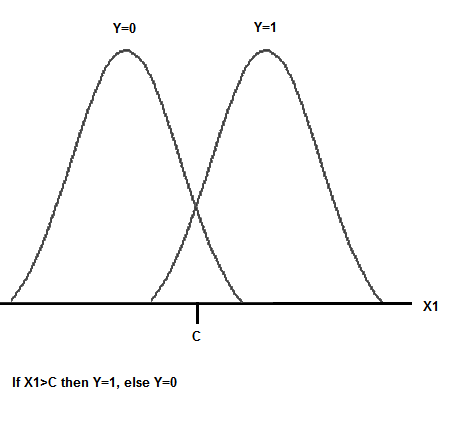
\includegraphics[width=0.5\textwidth]{Gaussians.png}
    \end{figure}
    
    \textbf{Select one:}
    \begin{checkboxes}
        \choice Yes, this can occur if the Gaussians are of equal means and equal variances.
        \choice Yes, this can occur if the Gaussians are of equal means and unequal variances.
        \choice Yes, this can occur if the Gaussians are of unequal means and equal variances. 
        \choice No, this cannot occur regardless of the relationship of the means or variances.
    \end{checkboxes}

    
    
    \clearpage
    
    \item \textbf{[4 pt]} Suppose that $0.3\%$ people have cancer. Someone decided to take a medical test for cancer. The outcome of the test can either be positive (cancer) or negative (no cancer). The test is not perfect - among people who have cancer, the test comes back positive 97\% of the time. Among people who don’t have cancer, the test comes back positive 4\% of the time. For this question, you should assume that the test results are independent of each other, given the true state (cancer or no cancer). What is the probability of a test subject having cancer, given that the subject’s test result is positive?
    
    If your answer is in decimals, answer with precision 4, e.g. (6.051, 0.1230, 1.234e+7)

    \textbf{Fill in the blank:}
    
    \begin{tcolorbox}[fit,height=1cm, width=4cm, blank, borderline={1pt}{-2pt},nobeforeafter]
    
    %solution
    \end{tcolorbox}
    
    
    \item \textbf{[4 pt]} In a Naive Bayes problem, suppose we are trying to compute $P(Y\mid X_1,X_2,X_3,X_4)$ .  Furthermore, suppose  $X_2$  and  $X_3$  are identical (i.e., $X_3$  is just a copy of $X_2$ ).  Which of the following are true in this case?

    \textbf{Select all that apply:}
    {\checkboxchar{$\Box$} \checkedchar{$\blacksquare$}
        \begin{checkboxes}
        \choice Naive Bayes will learn identical parameter values for $P(X_2|Y)$ and $P(X_3|Y)$.
        \choice Naive Bayes will output probabilities $P(Y|X_1,X_2,X_3,X_4)$ that are closer to 0 and 1 than they would be if we removed the feature corresponding to $X_3$.
        \choice This will not raise a problem in the output  $P(Y|X_1,X_2,X_3,X_4)$ because the conditional independence assumption will correctly treat this situation.
        \choice None of the above
    \end{checkboxes}
    }
    
    \item \textbf{[3 pt]} Which of the following machine learning algorithms are probabilistic generative models?

    \textbf{Select one:}
    \begin{checkboxes}
        \choice Decision Tree
        \choice K-nearest neighbors
        \choice Perceptron
        \choice Naive Bayes
        \choice Logistic Regression
        \choice Feed-forward neural network
    \end{checkboxes}
    

\clearpage

\item \textbf{[6 pt]} Logistic Regression and Naive Bayes. 
% \section*{Logistic Regression and Naive Bayes.}

When Y is Boolean and $\Xv = \langle{X_{1}...X_{n}}\rangle$ is a vector of continuous variables, then the assumptions of the Gaussian Naive Bayes classifier imply that $P(Y \mid \Xv)$ is given by the logistic function with
appropriate parameters $w_i$ for all $i$ and $b$. In particular:

\begin{align*}
    P(Y=1\mid\Xv)=\frac{1}{1+\exp(b+\sum_{i=1}^{n} w_iX_i)}
\end{align*}
and
\begin{align*}
    P(Y=0\mid\Xv)=\frac{\exp(b+\sum_{i=1}^{n} w_iX_i)}{1+\exp(b+\sum_{i=1}^{n} w_iX_i)}
\end{align*}

 Consider instead the case where Y is Boolean and ${\Xv = \langle{X_{1}...X_{n}}}\rangle$ is a vector
of Boolean variables.


Since the $X_{i}$ are Boolean variables, you need only one parameter to define $P(X_{i}\mid{Y} = y_k)$. Define $\phi_{i1} \equiv P(X_{i} = 1\mid{Y = 1})$, in which case $P(X_{i} = 0\mid{Y = 1}) = (1-\phi_{i1}$). Similarly, use $\phi_{i0}$ to denote $P(X_{i} = 1|Y = 0)$. 

\begin{enumerate}
    \item Given that we can simplify 
        
        $P(Y=1|X) = \frac{1}{1+\exp(ln(\frac{1-\pi}{\pi}) +\sum_i X_iln(\phi_{i0}) + ln(1-\phi_{i0}) - X_iln(1-\phi_{i0}) - X_iln(\phi_{i1}) - ln(1-\phi_{i1}) + X_iln(1-\phi_{i1}))}$ 
        
        Find expressions for $P(Y=1|X)$ and $P(Y=0|X)$ in terms of $b$ and $w_i$. Explicitly define $b$ and $w_i$.
        
        \begin{tcolorbox}[fit,height=10cm, blank, borderline={1pt}{-2pt},nobeforeafter]
    
    %solution
    \end{tcolorbox}
        
\end{enumerate}


\end{enumerate}

\clearpage





 \clearpage


\clearpage


\begin{comment} 
{\bf Collaboration Questions} After you have completed all other components of this assignment, report your answers to the collaboration policy questions detailed in the Academic Integrity Policies found \href{http://www.cs.cmu.edu/~mgormley/courses/10601-s18/about.html#7-academic-integrity-policies}{here}.
    \begin{enumerate*}
        \item Did you receive any help whatsoever from anyone in solving this assignment? If so, include full details.
        \item Did you give any help whatsoever to anyone in solving this assignment? If so, include full details?
        \item Did you find or come across code that implements any part of this assignment ? If so, include full details.
    \end{enumerate*}
    
    \begin{tcolorbox}[fit,height=3cm,blank, borderline={1pt}{-2pt},nobeforeafter]
    %Input your solution here.  Do not change any of the specifications of this solution box.
    \end{tcolorbox}
\end{comment}


\textbf{Collaboration Questions} Please answer the following:


    After you have completed all other components of this assignment, report your answers to the collaboration policy questions detailed in the Academic Integrity Policies found \href{http://www.cs.cmu.edu/~mgormley/courses/10601bd-f18/about.html#7-academic-integrity-policies}{here}.
    \begin{enumerate}
        \item Did you receive any help whatsoever from anyone in solving this assignment? Is so, include full details.
        \item Did you give any help whatsoever to anyone in solving this assignment? Is so, include full details.
        \item Did you find or come across code that implements any part of this assignment ? If so, include full details.
    \end{enumerate}
    
    \begin{solution}
    % If you are using the latex template, remove the empty spaces
    \bigskip \bigskip \bigskip \bigskip \bigskip \bigskip \bigskip \bigskip
    \bigskip \bigskip \bigskip \bigskip \bigskip \bigskip \bigskip \bigskip
    \bigskip \bigskip \bigskip \bigskip \bigskip \bigskip \bigskip \bigskip
    \bigskip \bigskip \bigskip \bigskip \bigskip \bigskip \bigskip \bigskip
    \bigskip \bigskip \bigskip \bigskip \bigskip \bigskip \bigskip \bigskip
    \bigskip \bigskip \bigskip \bigskip \bigskip \bigskip \bigskip \bigskip
    \bigskip \bigskip \bigskip \bigskip \bigskip \bigskip \bigskip \bigskip
    \end{solution}
    

\end{document}
